% 目次の挿入
\tableofcontents
\newpage

% ヘッダーカスタマイズ
\pagestyle{fancy}
\fancyhf{}
\fancyhead[L]{DLITE3:Technology that supports people's lives without boundaries}
\renewcommand{\headrulewidth}{0pt}
\makeatletter
\let\ps@plain\ps@fancy
\makeatother

\chapter{はじめに}
\section{背景}
Describe the background here.\cite{テスト}
\Writer{未来太郎}

\section{方法}
Describe the methods used here.

\section{結果}
Summarize the results here.

\begin{figure}[h!]
  \centering
  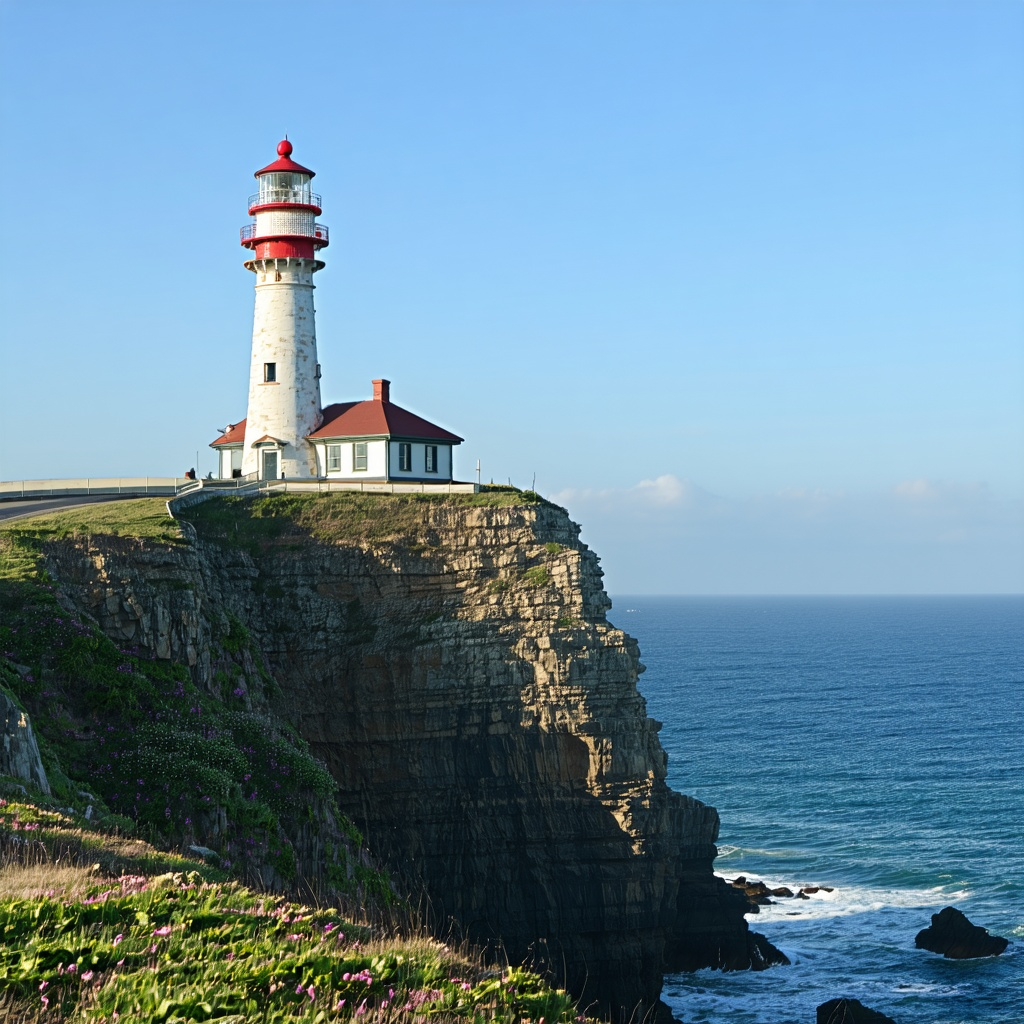
\includegraphics[width=0.8\textwidth]{pages/report/images/sample.jpg}
  \caption{Sample Image Description}
  \label{fig:sample}
\end{figure}

\newpage\clearpage
\vspace*{15pt}
\addcontentsline{toc}{chapter}{参考文献}  % 目次に「参考文献」を追加
\printbibliography[segment=\therefsegment,heading=subbibliography]
